\documentclass{llncs}
\usepackage{amssymb}
\usepackage{graphicx}
\usepackage[ruled,linesnumbered,boxed]{algorithm2e}
\usepackage{graphicx}
\usepackage{amsmath}
%\usepackage{mathtools}
%\usepackage{color}
\usepackage{tabularx}
\usepackage[colorlinks, linkcolor=blue, anchorcolor=blue, citecolor=green]{hyperref}
%\usepackage{booktabs}
\usepackage[table]{xcolor}
%\uespackage{colortbl}
\usepackage[tight,footnotesize]{subfigure}
\usepackage{fancyhdr}
\usepackage{lastpage}
\usepackage{layout}
\usepackage{appendix}
%\usepackage{ctex}
\usepackage{float}
\usepackage{multirow}
\usepackage{booktabs}
\usepackage{comment}

\usepackage{indentfirst}
\setlength{\parindent}{2em}

%\footskip = 10pt
\pagestyle{fancy}
\chead{Group Project}
\lhead{CS2308-Algorithm@SJTU}
\rhead{Instructor: Xiaofeng Gao}
\rfoot{}
\cfoot{Page \thepage \ of \pageref{LastPage}}
\addtolength{\headheight}{0.5\baselineskip}
\addtolength{\headwidth}{0\marginparsep}
\addtolength{\headwidth}{0\marginparwidth}



\title{Resource Scheduling Problem in Hadoop}
\subtitle{\color{blue}{Project for Algorithm and Complexity Course} \vspace{-6mm}}

\author{}
\institute{Department of Computer Science and Engineering, \\ Shanghai Jiao Tong University, Shanghai, China}

\begin{document}
\bibliographystyle{plain}

%\linespread{0.85}

%==============================================================================
\maketitle
\begin{abstract}\vspace{-5mm}

The course project focuses on resource scheduling problem in Hadoop. This document introduce the background and two versions of resource scheduling on single or multiple hosts. Also, it lists all the tasks and requirements for each student group. Please read this document carefully and complete the corresponding tasks.

\textbf{Keywords:} Distributed Computing System, Resource Scheduling, Hadoop
\end{abstract}

\section{Background and Motivation}
\label{sec-Hadoop}

Hadoop is an open-source software framework for storing data and running applications on clusters of commodity hardware. In Hadoop, the data of a running job can be divided into several data blocks, stored on different hosts. Each host has one or multiple CPU cores to process data blocks. In this project, our goal is to achieve effective parallel computing. That is to say, given a set of jobs with massive data, we need to design a resource scheduling algorithm to minimize the overall executing time of all jobs.



\section{A Simplified Version with Single Host}
\label{sec-problem1}

First, let us consider a simple case with a single host storing all data blocks. Please read the assumptions, specifications, symbol notations, constraints, and explanations in Subsection~\ref{subsec-preliminary} carefully and then complete the tasks mentioned in Subsection~\ref{subsec-single}.

\subsection{Problem Formulation and Explanation} \label{subsec-preliminary}

To simplify the problem, we give the following assumptions and specifications.

\begin{enumerate}

  \item There are $n$ jobs that need to be processed by a single host, which has $m$ CPU cores of the same computing capability. Let $J$ be the set of jobs, and $C$ be the set of cores for the host, where $J = \{job_0, job_1, \cdots, job_{n-1}\}$, and $C = \{c_0, c_1, \cdots, c_{m-1}\}$ (The labels of variables start from 0 because we use C/C++ source codes in the following tasks).
  
  \vspace{2mm} 
  
  \item We treat data block as the smallest indivisible unit in our project, while a job can be divided into multiple data blocks with different sizes for storage and computing. Assume $job_i$ is split into $n_i$ data blocks, denoted by $B^i = \{b^i_{0}, b^i_{1}, \cdots, b^i_{n_i-1}\}$. For block $b^i_{k}$ of $job_i$, define its size as $size(b^i_{k})$.
  
  \vspace{2mm} 
  
  \item Assume $job_i$ is assigned to $e_i$ cores for processing, and naturally $e_i \leq n_i$. That is to say, one core can process multiple data blocks of one job sequentially. Let $B^i_{j}\subseteq B^i$ denote the set of data blocks of $job_i$ allocated to core $c_j$, and $B^i_{j} \cap B^i_{j'} = \varnothing$ if $j \neq j'$ (they should be disjointed). 
  
  \vspace{2mm} 
  
  \item For $job_i$, the processing speed of its data blocks is $s_i$ when $job_i$ is assigned to a single core. However, when multiple cores process $job_i$ in parallel, the computing speed of each core all decays because of some complicated interactions. We formulate such speed decay effect caused by multi-core computation as a coefficient function $g(\cdot)$ with respect to core number $e_i$, as described in Equation~\eqref{Eq-decay}:
    \begin{equation} \label{Eq-decay}
    g (e_i) = 1.00 - \alpha \cdot (e_i-1), \quad  \text{for} \ 1 \leq e_i \leq 10,
    \end{equation}
  where $\alpha$ is a decay factor satisfying $0 < \alpha < 1$ , and usually the number of cores for processing a single job is no more than 10. Then, the speed of each core can be rewritten as $s_i \cdot g(e_i)$ for $job_i$ respectively. (Note that although the speed of each core decays, the overall processing time using $e_i$ cores in parallel should be faster than that of using just one core. Otherwise we do not need to implement parallel computing. Thus the setting of $\alpha$ should guarantee this principle.)
  
  \qquad Correspondingly, the processing time $tp^i_{j}$ of core $c_j$ for $job_i$ can be expressed as Equation~\eqref{Eq-process}:
  \begin{equation} \label{Eq-process}
  tp^i_{j} = \frac{\sum_{b^i_{k} \in B^i_{j}}size(b^i_{k})}{s_i \cdot g(e_i)}.
  \end{equation} 
  
  \vspace{2mm}

  \item For consistency issues, if we assign a job to multiple cores, all cores must start processing data blocks at the same time. If one or several cores are occupied by other affairs, then all other cores should wait for a synchronous start, and keep idle. It means that the processing of $job_i$ for every core should all start at time $t_i$, whereas their processing duration might be different. Let $tf^i_{j}$ be the finishing time of core $c_j$ for $job_i$, which is calculated by Equation~\eqref{Eq-finish}:
  \begin{equation} \label{Eq-finish}
  tf^i_{j} = t_i + tp^i_{j}.
  \end{equation}   
  
  However, the occupied cores of $job_i$ are released synchronously when the computing process of the last data block is finished. Thus the finishing time $tf(job_i)$ of $job_i$ is given as Equation~\eqref{Eq-jobfinish}:
  \begin{equation} \label{Eq-jobfinish}
  tf(job_i) = \max_{c_j} \; tf^i_{j}, \text{ for } c_j \in C.
  \end{equation} 
\end{enumerate}


Please keep these assumptions and specifications in mind and finish the following tasks.


\subsection{Task 1: Resource Scheduling for Single Host} \label{subsec-single}

Based on the descriptions in Subsection~\ref{subsec-preliminary}, your work is to design a resource scheduling algorithm to minimize the overall finishing time of all jobs, whose objective function is shown as:
  \begin{equation*}
  \min \max_{job_i} tf(job_i), \ \text{ for } job_i \in J. 
  \end{equation*}  

Figure~\ref{Fig-SingleHostExample} illustrates a toy example of scheduling resources among three jobs $job_0, job_1$, $job_2$ on a single host, which has four cores $c_0, c_1, c_2, c_3$. All blocks of $job_0, job_1$, and $job_2$ are stored on this host, with different sizes measured by megabyte (MB). The goal is to find a scheduling strategy assigning data blocks to suitable cores so that the overall finishing time of three jobs is minimized.


\begin{figure}[htbp]
\centering
\begin{minipage}[t]{0.38\textwidth}
\centering
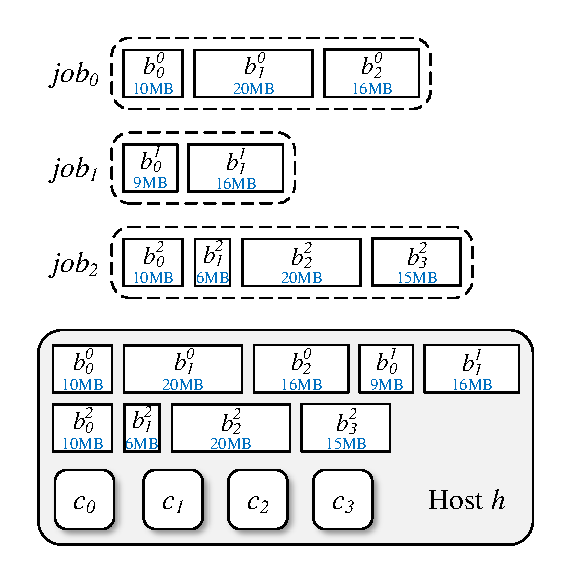
\includegraphics[width=\textwidth]{Fig-SingleHostExample.pdf}
\caption{A toy example of scheduling resources for a single host}
\label{Fig-SingleHostExample}
\end{minipage}
\begin{minipage}[t]{0.6\textwidth}
\centering
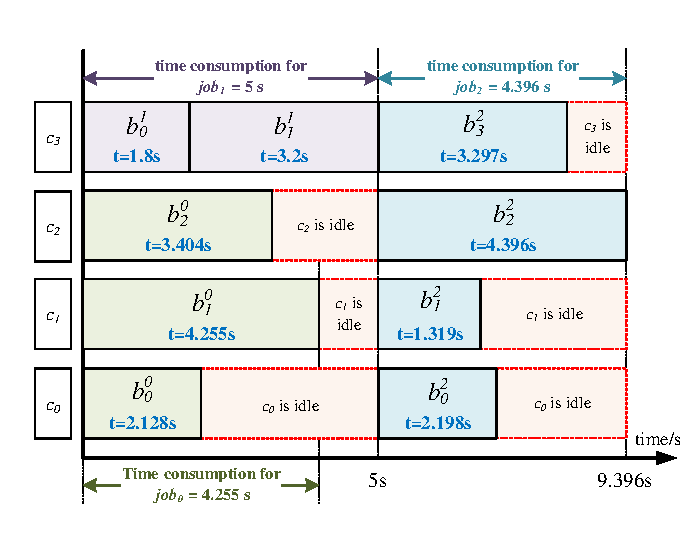
\includegraphics[width=\textwidth]{Fig-SingleHostResult.pdf}
\caption{Time consumption of a feasible solution for the example in Figure \ref{Fig-SingleHostExample}}
\label{Fig-SingleHostResult}
\end{minipage}
\end{figure}


\emph{Remark}. Assume the sizes of three blocks of $job_0$ are respectively $size(b^0_0)=10$ MB, $size(b^0_1)=20$ MB and $size(b^0_2) = 16$ MB, while those of $job_1$ are $size(b^1_0) = 9$ MB and $size(b^1_1) = 16$ MB. The size of each block in $job_2$ is $size(b^2_0) = 10$ MB, $size(b^2_1) = 6$ MB, $size(b^2_2) = 20$ MB and $size(b^2_3) = 15$ MB, respectively. Moreover, suppose the computing speed is $s_i=5$ MB/s for $i = 0$, 1, 2, and $\alpha = 0.03$ to compute the decay coefficient $g(\cdot)$ in Equation~\eqref{Eq-decay}.

Here we provide a feasible solution (as shown in Figure~\ref{Fig-SingleHostResult}) for the above setting in Figure \ref{Fig-SingleHostExample}, in which blocks of $job_0$ are assigned to three cores $c_0$, $c_1$, $c_2$, and blocks of $job_1$ are assigned to the last core $c_3$. Now, we can compute the processing time of core $c_0$, $c_1$, $c_2$ for $job_0$ as Equation~\eqref{Eq-job0} respectively:
\begin{equation} \label{Eq-job0}
\left\{
\begin{array}{ccl}
 tp^0_0  & = &  size(b_0^0)/(s_0\cdot g(e_0))=10 / (5 \times (1.00 - 0.03 \times (3-1))) = 2.128\text{s},\\
 tp^0_1  & = & size(b_1^0)/(s_0\cdot g(e_0)) = 20/4.7 = 4.255\text{s},\\
 tp^0_2 & = & size(b_2^0)/(s_0\cdot g(e_0)) = 16/4.7 = 3.404\text{s}.
\end{array}
\right.
\end{equation}

Moreover, the processing of $job_0$ starts at $0$s, so the finishing time of $job_0$ is $$tf(job_0) =0+ \max \{ tp^0_0, tp^0_1, tp^0_2\} = \max \{2.128, 4.255, 3.404\} = 4.255\text{s}.$$ The processing time of blocks $b^1_0$ and $b^1_1$ with the single core $c_3$ is $t^1_0 = 9/5 = 1.8$s and $t^1_1 = 16/5 = 3.2$s, respectively. Then the finishing time of $job_1$ is $tf(job_1) = 1.8 + 3.2 = 5$s.

We assign $job_2$ to four cores, each of which should start after $job_1$ releases the occupied core. Obviously, the processing of $job_2$ starts at $5$s. The processing time of each block of $job_2$ is: 
\begin{equation*}
\left\{
\begin{array}{ccl}
 t^2_0 & = & size(b^2_0)/(s_2\cdot g(e_2))=10 / (5 \times (1.00 - 0.03 \times (4-1))) = 2.198\text{s},  \\
 t^2_1 & = & size(b^2_1)/(s_2\cdot g(e_2)) = 6/4.55 = 1.319\text{s}, \\
 t^2_2 & = & size(b^2_2)/(s_2\cdot g(e_2))= 20/4.55 = 4.396\text{s}, \\
 t^2_3 & = & size(b^2_3)/(s_2\cdot g(e_2))= 15/4.55 = 3.297\text{s}.
\end{array}
\right.
\end{equation*}


Then we can get that the finishing time of $job_2$ as $$tf(job_2) = 5 + \max\{ 2.198, 1.319, 4.396, 3.297\} = 9.396\text{s}.$$ Thus, the overall finishing time of the three jobs is $$\max\{tf(job_0), tf(job_1), tf(job_2) \} = 9.396\text{s}.$$ It is observed that for a multi-core job, its time consumption is determined by the last completed block, while for the whole system, the total finishing time is decided by the last finished job. However, Figure~\ref{Fig-SingleHostResult} is just a feasible solution and not necessarily optimal, since cores $c_0$, $c_1$, $c_2$, and $c_3$ are all idle for a while during the whole process, which is a waste of resources. 

\vspace{2mm}

Based on the above explanations and examples, please finish the following tasks:
\begin{enumerate}
  \vspace{-1mm}
  \item Formalize the resource scheduling problem for a single host as a programming pattern with objective function and constraints. You cannot rename the variables that have been defined in the project, whereas you are free to introduce other new variables, and please define your variables clearly.
  
  \item Please design an algorithm to solve this problem efficiently. First, describe your idea in detail, and then provide the corresponding pseudocode. Also, please discuss the time complexity of your design.
  \item Verify your algorithm using the attached test data in ``task1\underline\ case1.txt'' under $input$ file folder and save your result in the .txt file, named as ``task1\underline\ case1\underline\ TeamNumber.txt'' (e.g., task1\underline\ case1\underline\ 06.txt). The input/output format is fixed in the reference codes. Optionally, visualize your result while the visual format is not limited. For example, you can plot a figure from the perspective of cores on the host. The test data and reference codes are also released on GitHub: \href{https://github.com/shiwanghua/SharedFiles/tree/Project-CodeDemo}{Resource Scheduling Problem}.
\end{enumerate}


\section{A Comprehensive Version among Multiple Hosts}
\label{sec-problem2}

In this section, we consider a more complex situation, where we need to schedule resources among multiple hosts. Now the data transmission process between pairwise hosts should be taken into consideration. The data blocks of jobs could be initially stored on different hosts, but one data block can only be initially stored on one specified host. If data block $b^i_{k}$ and its assigned computing core $c_j$ are not on the same host, $b^i_{k}$ will be transmitted to the host containing $c_j$ (Here we assume that the bandwidth between hosts is sufficient for data transmission). The transmission process will influence the finishing time of jobs, further affecting the resource scheduling process.

\subsection{Problem Formulation and Explanation}

Besides the descriptions and specifications of Task 1, here are more notations and explanations.

\begin{enumerate}

  \item Assume we have $q$ hosts $H=\{h_0, h_1, \cdots, h_{q-1}\}$, and host $h_l$ has $m_l$ cores (may have different number of cores). Let $C_l$ be the set of cores on host $h_l$, $C_l = \{c^l_0, c^l_1, \cdots, c^l_{m_l-1}\}$. Easy to see, $\sum_{l=0}^{q-1} m_l = m$.
  
  \vspace{2mm}

  \item If core $c^l_j$ on host $h_l$ computes a data block $b^i_{k}$ of $job_i$ which is initially stored on another host $h_l'$, then $b^i_{k}$ needs to be transmitted from $h_l'$ to $h_l$ at a transmission speed $s_t$ (this speed is fixed in our system). An example is shown in Figure~\ref{Fig-Transmission}, where hosts $h_0$ and $h_1$ both have two cores, and many jobs need to be processed. Core $c^1_0$ on host $h_1$ is assigned to compute the data block $b^1_2$ of $job_1$, which is initially stored on host $h_0$. In this case, $b^1_2$ needs to be transmitted from $h_0$ to $h_1$ at a transmission speed $s_t$ first, and then be computed by $c^1_0$. Whenever $b^1_2$ starts transmission, other cores can work in parallel to process $job_1$.
  
  \begin{figure}[H]
  \begin{center}
  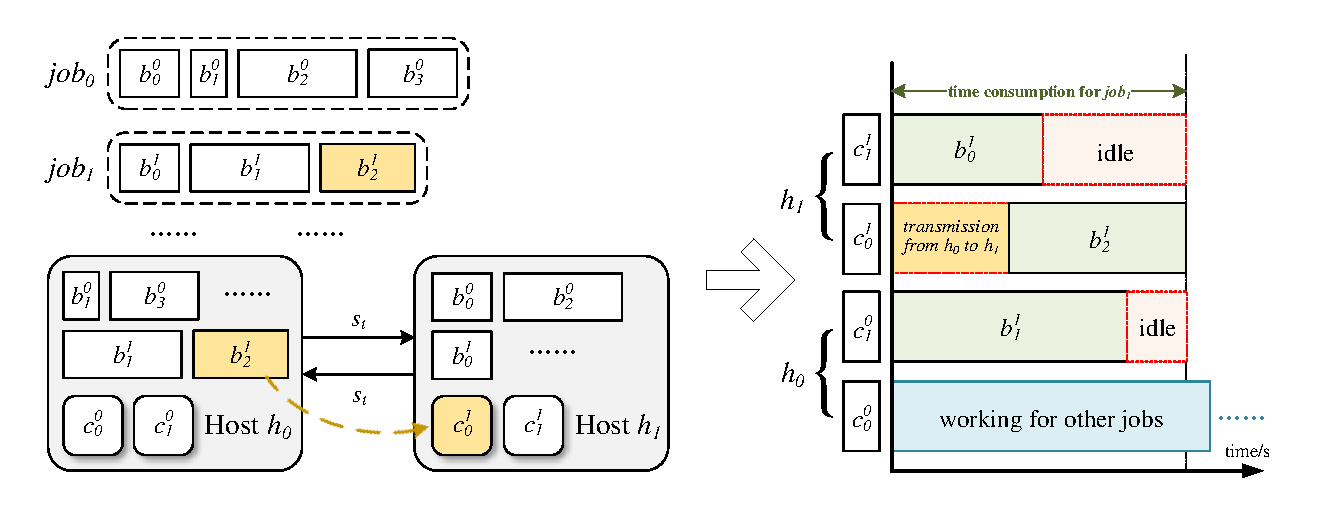
\includegraphics[width=0.9\textwidth]{Fig-Transmission.pdf}
  \caption{An example of data transmission between 2 hosts}
  \label{Fig-Transmission}
  \end{center}
  \end{figure}

  \item Any core cannot call for data transmission when it is calculating other data blocks. Likewise, a core cannot start computing any data block until this block is ready, i.e. initially on the same host or transmitted from a remote host to the local host. For example, the core $c^1_0$ on host $h_1$ must wait for the data transmission of block $b^1_2$ from host $h_0$ to $h_1$, and then start computation. What is more, the transmission time of $b^1_2$ from $h_0$ to $h_1$ affects the finishing time of $job_0$, further affecting the finishing time of the whole system. 
  
  \qquad For core $c^l_j$ on host $h_l$, let $\widetilde{B}^i_{lj}$ be the set of data blocks of $job_i$ allocated to $c^l_j$ but not initially stored on host $h_l$. All the data blocks in $\widetilde{B}^i_{lj}$ need to be transmitted to host $h_l$ before computing. Let $B^i_{lj}$ be the set of data blocks of $job_i$ allocated to core $c^l_j$. Then, the processing time $tp^i_{lj}$ of core $c^l_j$ for $job_i$ can be reformulated as Equation~\eqref{Eq-tptransmission}:
  \begin{equation} \label{Eq-tptransmission}
  tp^i_{lj} = \frac{\sum_{b^i_{k} \in \widetilde{B}^i_{lj}} size(b^i_{k})}{s_t} + \frac{\sum_{b^i_{k} \in B^i_{lj}}size(b^i_{k})}{s_i \cdot g(e_i)}.
  \end{equation}
  
 \item If the processing of $job_i$ starts at time $t_i$, then the finishing time of core $c^l_j$ for $job_i$ is
  \begin{equation*}
  tf^i_{lj} = t_i + tp^i_{lj}.
  \end{equation*}
  
  Then the finishing time $tf(job_i)$ of $job_i$ is formulated as:
  \begin{equation*}
  tf(job_i) = \max_{c^l_j} \; tf^i_{lj}, \text{ for } c^l_j \in C.
  \end{equation*}

\end{enumerate}

Please keep these assumptions and specifications in mind and finish the following tasks.

\subsection{Task 2: Resource Scheduling among Multiple Hosts}

Similarly, the aim of Task 2 is to design a resource scheduling algorithm among multiple hosts to minimize the overall finishing time, which is formulated as:
  \begin{equation*}
  \min \max_{job_i} tf(job_i), \text{ for } job_i \in J.
  \end{equation*}  

Figure \ref{Fig-MultiHostExample} shows a toy example of scheduling resources among 3 hosts. We have 4 different jobs, each of which consists of blocks with different sizes. For example, $job_0$ has three blocks, $b^0_1$, $b^0_1$, and $b^0_2$, stored on host $h_0$. Other jobs are stored on different hosts. These data blocks are assigned to available cores on the three hosts, each with \textbf{two} cores. Then this scheduling should consider the data transmission process if the data block and its allocated core are not on the same host. Our goal is to find a scheduling strategy to allocate data blocks to appropriate cores so that the overall finishing time of four jobs is minimized.

\begin{figure}[H]
\begin{center}
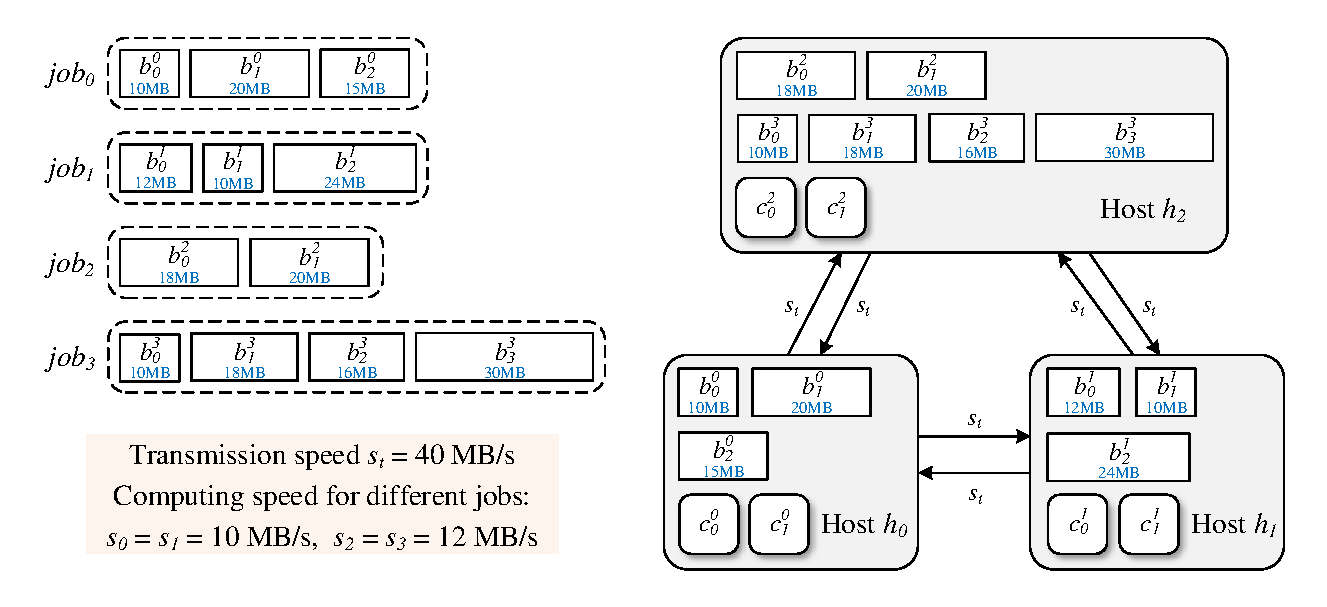
\includegraphics[width=0.9\textwidth]{Fig-MultiHostExample.pdf}
\caption{A toy example of scheduling resources among 3 hosts}\label{Fig-MultiHostExample}
\end{center}
\end{figure}



\begin{figure}[htbp] 
%\centering    
\begin{center}
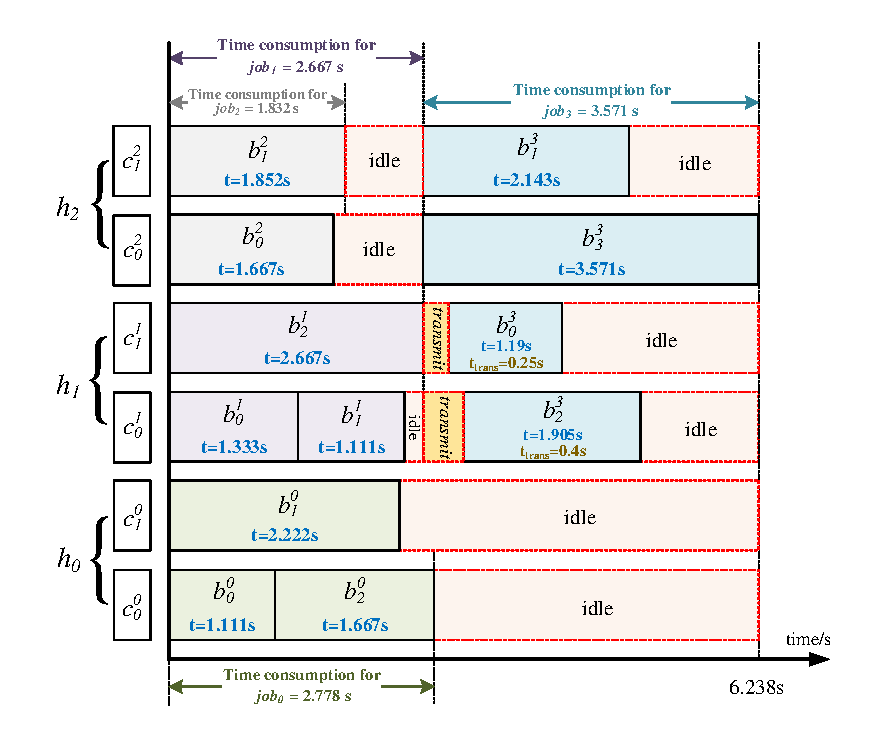
\includegraphics[width=0.7\textwidth]{Fig-MultiHostResult.pdf}
\caption{Time consumption of a feasible solution for the example in Figure~\ref{Fig-MultiHostExample}.}
\label{Fig-MultiHostResult}
\end{center}
\end{figure}

\emph{Remark}. Assume the sizes of three blocks of $job_0$ are respectively set as $size(b_0^0)=10$ MB,
$size(b^0_1) = 20$ MB and $size(b^0_2) = 15$ MB, while those of other jobs are listed in the left hand of Figure \ref{Fig-MultiHostExample}. Set decay factor $\alpha = 0.1$, and then the computing decaying coefficient is $g(e_i)=1-0.1\times(e_i-1)$. Besides, we set the transmission speed as $s_t = 40$ MB/s. Assume that $job_0$ and $job_1$ have the same computing speed, which is $s_0 = s_1= 10$ MB/s. Similarly, the computing speed of $job_2$ and $job_3$ is $s_2 = s_3= 12$ MB/s. Under the above settings, we give a feasible solution for the example in Figure~\ref{Fig-MultiHostExample}, as shown in Figure~\ref{Fig-MultiHostResult}.

In the initialization phase, we know that blocks of $job_0$ are on the host $h_0$, blocks of $job_1$ are on $h_1$, blocks of $job_2$ and $job_3$ are on $h_2$. Thus we choose to compute $job_0$, $job_1$, and $job_2$ on their own local host, each with two cores.

Firstly, the calculation of time consumption is similar to the example of Task 1. For instance, the time consumption of block $b^2_0$, also the processing time of core $c^2_0$ for $job_2$, is 
\begin{equation}
\begin{aligned}
{tp}^2_{21}=\frac{size(b^2_0)}{s_2\times{g(e_2)}}=\frac{18}{12\times{g(2)}}=\frac{18}{12\times0.9}=1.667\text{s}.
\label{Eq-time-multi}
\end{aligned}
\end{equation}

As shown in Equation~\eqref{Eq-time-multi}, we can compute the time consumption of the rest blocks in $job_0$, $job_1$ and $job_2$. One job can be allocated to multiple cores on different hosts and each block of this job can be computed by only one core. We allocate the data blocks of $job_2$ to cores $c^2_0$ and $c^2_1$ for computing. In detail, $c^2_0$ computes $b^2_0$ and $c^2_1$ computes $b^2_1$. Cores $c^2_0$ and $c^2_1$ must be released simultaneously when the computing of $b^2_1$ is finished. Thus, the finishing time of $job_2$ in this stage is $1.852s$, while $c^2_0$ and $c^2_1$ stay idle to wait for new task allocation.

In the same way, $job_0$, $job_1$, and $job_2$ have been allocated to certain cores to finish computing. As shown in Figure \ref{Fig-MultiHostResult}, 4 cores on $h_1$ and $h_2$ stay in idle state after finishing the computation of $c^1_1$. We consider that allocating $job_3$ to 4 cores on $h_1$ and $h_2$ is feasible.

When the system allocates $job_3$ to 4 cores and starts processing it, it is \textbf{necessary} to transmit the blocks of $job_3$ from host $h_2$ to host $h_1$. According to the actual condition, the time of job computing starting is the time of transmission starting. For instance, 4 blocks of $job_3$ are allocated to 4 cores for computing. We can compute $b^3_1$ and $b^3_3$ at local host directly, rather transmit $b^3_0$ and $b^3_2$ to host $h_1$. The transmission time for $b^3_0$ can be calculated as $\frac{size(b^3_0)}{s_t}=\frac{10}{40}=0.25$s.

\begin{comment}
\begin{equation}
\begin{aligned}
{t_T}^3_0=\frac{size(b^3_0)}{s_t}=\frac{10}{40}=0.25s
\label{trans-time}
\end{aligned}
\end{equation}
\end{comment}


Consequently, the time consumption of $b^3_0$, also the processing time of core $c^1_1$ for $job_3$, could be computed as Equation~\eqref{Eq-time-all}.

\begin{equation}
\begin{aligned}
{tp}^3_{11}=0.25+\frac{size(b^2_0)}{s_3\times{g(e_3)}}=0.25+\frac{10}{12\times{g(4)}}=0.25+\frac{10}{12\times0.7}=1.440\text{s}.
\label{Eq-time-all}
\end{aligned}
\end{equation}

It is the same as the above that some cores could be in idle state when finishing block computing. Thus, the processing time of $job_3$ in this stage is the time consumption of $b^3_3$, which is $3.571$s. The whole time consumption of this example is the latest finishing time of all jobs, which is calculated to be $6.238$s. Figure \ref{Fig-MultiHostResult} shows the time consumption of this solution and the red dotted box expresses the idle state of cores during the scheduling process.

Obviously, the time consumption of this solution could utilize resources as much as possible, which means that the data transmission can affect the final overall finishing time. However, what is remarkable is that the solution given in Figure~\ref{Fig-MultiHostResult} may not be optimal for the example in Figure~\ref{Fig-MultiHostExample}. Because idle state indicates the resource waste and this solution can still be optimized.

\vspace{2mm}
Based on the above discussions and examples, please finish the following tasks:
\begin{enumerate}
  \vspace{-1mm}
  \item Formalize the resource scheduling problem among multiple hosts as a programming pattern with objective function and constraints. Justify whether it is an NP-Complete problem.
  \item Design an algorithm to solve this problem. First, describe your idea in detail, and then provide the corresponding pseudo code. Also, please discuss the time complexity of your design.
  \item Verify your algorithm using test data ``task2\underline\ case1.txt'' in $input$ file folder and save your result in the .txt file, named as ``task2\underline\ case1\underline\ TeamNumber.txt'' (e.g., ``task2\underline\ case1\underline\ 06.txt''). The input/output format is fixed in the reference codes. Optionally, visualize your result in an unlimited format. For example, you can plot a figure from the perspective of cores on the host. The test data and reference codes are also released on GitHub: \href{https://github.com/shiwanghua/SharedFiles/tree/Project-CodeDemo}{Resource Scheduling Problem}. 
\end{enumerate}


\section{Report Requirements}

You need to submit a report for this project, with the following requirements:

\begin{enumerate}
  \item Your report should include the title, the author names, IDs, email addresses, the page header, the page numbers, your results and discussions for the tasks, figures for your simulations, tables for discussions and comparisons, with the corresponding figure titles and table titles.
  
  \item Your report should be in English only, with a clear structure, divided by sections, and may contain organizational architecture such as items, definitions, or discussions.
  
  \item Please include Reference section and Acknowledgment section. You may also include your feelings, suggestions, and comments in the acknowledgment section.
  
  \item Please define your variables clearly and add them into the symbol table in Appendix.
  
  \item Please create a folder named ``Project-TeamNumber'', which contains related materials such as report ``Project-TeamNumber.pdf'', latex source ``Project-TeamNumber.tex'', the executable file ``Project-TeamNumber.exe'' (if you have), the data output folder ``Project-Outputs-TeamNumber'', the figure folder ``Project-Figures-TeamNumber'', and other code file folder  ``Project-Codes-TeamNumber''. Then compress the home folder ``Project-TeamNumber'' into a ``Project-TeamNumber.zip'' package. Note that TeamNumber should be two-digit number, e.g., ``Project-06.zip'' conforms to the rule.
\end{enumerate}





\section*{Acknowledgements}
This problem is motivated from a real-world cloud service corporation. It is formulated by Prof. Xiaofeng Gao (gao-xf@cs.sjtu.edu.cn) from Department of Computer Science and Engineering at Shanghai Jiao Tong University. Yue Ma scribed and modified the project. Yangyang Bao provided the example in Task 1. Zhen Sun provided the example in Task 2. Wanghua Shi provided the test data and source code. Jiale Zhang, Tianyao Shi helped on proofreading and provided many suggestions.

% Here is your acknowledgements. You may also include your feelings, suggestion, and comments in the acknowledgement section.

%
% ---- Bibliography ----
%
% BibTeX users should specify bibliography style 'splncs04'.
% References will then be sorted and formatted in the correct style.
%
%\bibliographystyle{splncs04}
% \bibliography{refpaper.bib}
%

%\newpage
\begin{appendices}
\section*{Appendix}

\begin{table}[htbp]
\caption{Symbols and Definitions}
\begin{center}
\begin{tabular}{c|c}
\toprule
\textbf{Symbols} &\textbf{Definitions}  \\
\midrule
$n$ & The number of jobs  \\ 
$m$ & The number of cores \\
$q$ & The number of hosts  \\ 
$job_i$, $J$ & $job_i$ is the $i$-th job. The job set is $J=\{job_0, \cdots, job_{n-1}\}$. \\ 
$h_l$, $H$ & $h_l$ is the $l$-th  host. The host set is $H=\{h_0, \cdots, h_{q-1}\}$. \\ 
$m_l$ & The number of cores on host $h_l$\\
$c^l_j$, $C_l$ & $c^l_j$ is the $j$-th core on host $h_l$. $C_l$ is the set of cores on host $h_l$.\\ 
$C$ & The set of cores. $C=\{c_0,\cdots,c_{m-1}\}$ for single-host. $C=\cup_{l=0}^{q-1} C_l$ for multi-host.\\
$b^i_k$& The block of $job_i$ whose id is $k$\\
$B^i_{j}$ & The set of data blocks of $job_i$ allocated to core $c_j$ \\
$B^i$ & The set of data blocks of $job_i$ \\ 
$B^i_{lj}$ & The set of data blocks of $job_i$ allocated to core $c^l_j$ \\
$\widetilde{B}^i_{lj}$ & The set of data blocks of $job_i$ allocated to core $c^l_j$ but not initially stored on $h_l$\\
$size(\cdot)$ & The size function of data block\\
$g(\cdot)$ &  The computing decaying coefficient caused by multi-core effect\\
$s_i$ & The computing speed of $job_i$ by a single core\\
$s_t$ & The transmission speed of data \\
$e_i$ & The number of cores processing $job_i$\\ 
$t_i$ & The time to start processing $job_i$\\
$tp^i_j$, $tf^i_{j}$ & The processing time / finishing time of core $c_j$ for $job_i$\\
$tp^i_{lj}$, $tf^i_{lj}$ & The processing time / finishing time of core $c^l_j$ for $job_i$\\
$tf(job_i)$ & The finishing time of $job_i$ \\
%  & \\
%  & \\
%  & \\
%  & \\
%  & \\
%  & \\ 
 
\bottomrule
%\multicolumn{4}{l}{$^{\mathrm{a}}$Sample of a Table footnote.}
\end{tabular}
\label{tabSYMBOLS}
\end{center}
\end{table}

\end{appendices}

%\begin{comment}
%\begin{thebibliography}{8}
%\bibitem{ref_article}
%Author, F.: Article title. Journal \textbf{2}(5), 99--110 (2016)
% \bibitem{dean2008mapreduce}
% Dean J, Ghemawat S. MapReduce: simplified data processing on large clusters[J]. Communications of the ACM, 2008, 51(1): 107-113.

% \bibitem{ref_lncs1}
% Author, F., Author, S.: Title of a proceedings paper. In: Editor,
% F., Editor, S. (eds.) CONFERENCE 2016, LNCS, vol. 9999, pp. 1--13.
% Springer, Heidelberg (2016).

% \bibitem{ref_book1}
% Author, F., Author, S., Author, T.: Book title. 2nd edn. Publisher,
% Location (1999)

% \bibitem{ref_proc1}
% Author, A.-B.: Contribution title. In: 9th International Proceedings
% on Proceedings, pp. 1--2. Publisher, Location (2010)

% \bibitem{ref_url1}
% LNCS Homepage, \url{http://www.springer.com/lncs}. Last accessed 4
% Oct 2017
%\end{thebibliography}
%\end{comment}

\end{document}


